\section{The Big Idea}
 \begin{wrapfigure}{r}{0.14\columnwidth}
	\vspace{-4em}
		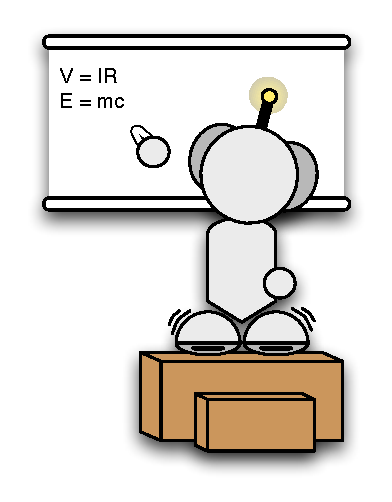
\includegraphics[width=0.14\columnwidth, trim=20mm 10mm 10mm 10mm]{diagrams/robot_whiteboard.pdf}
 	\vspace{-2em}
 \end{wrapfigure}
Pathfinding often involves exploring highly regular 
environments such as cities, sewers or dungeons; see e.g Figure \ref{fig:iw2}.
Though these locales tend to be topographically simple (usually being comprised
of empty rooms connected by corridors) they can also be highly symmetric 
with many optimal length paths existing between arbitrary pairs of locations.
Symmetry is undesirable as it increases the size of the search space and forces
search algorithms to waste time \cite{walsh07}.
\newline \newline
We propose the following offline strategy for identifying and eliminating symmetric paths in 
4-connected grid maps:
\newline \newline
1. Decompose the grid map into a set of empty rectangular rooms.
\newline
2. Prune all tiles not on the perimeter of an empty room.
\newline
3. Connect each tile on the perimeter with the tile on the directly opposite side of the room.
\newline \newline
Sometimes a tile which has been pruned is later required; for example as a start
or goal location. 
We handle these cases by temporarily re-inserting the required tile back into
the grid map and connecting it with the closest node on each side the perimeter.
\newline \newline
Figure \ref{fig:splash} shows an example of this process.
It is easy see to see that we eliminate a large number of symmetric paths
that between arbitrary pairs of tiles on the perimeter of each room. 
Furthermore, we can prove that for each optimal length path in the
original grid map there is an equivalent length path in our pruned grid map.
